\section{Proposed solution}
\label{sec:proposedsolution}
With the objective of monitoring the temperature of a given area - e. g. a piggery, the scenario is as follows: A number of similar sensor nodes is distributed around the area each connected to the same network. This network is in this project capable of providing a reliable channel through TCP. A \textit{user}-entity chooses one sensor node to be the admin node. 

As depicted in Figure \ref{fig:overview} the execution of the system can be devided into 3 main categories:
\begin{description}
    \item[Reporting] Regular nodes reports their temperature to the admin node periodically.
    \item[User request] Upon request, the admin node evaluates the average temperature from the available data that is not too old and returns the result.
    \item[Promote new master] When an admin node crashes or other wise fall out of service, the user then selects and promotes a regular node, which in turn notifies the remaining regular nodes of the promotion.
\end{description}
\begin{figure}[ht!]
\centering
    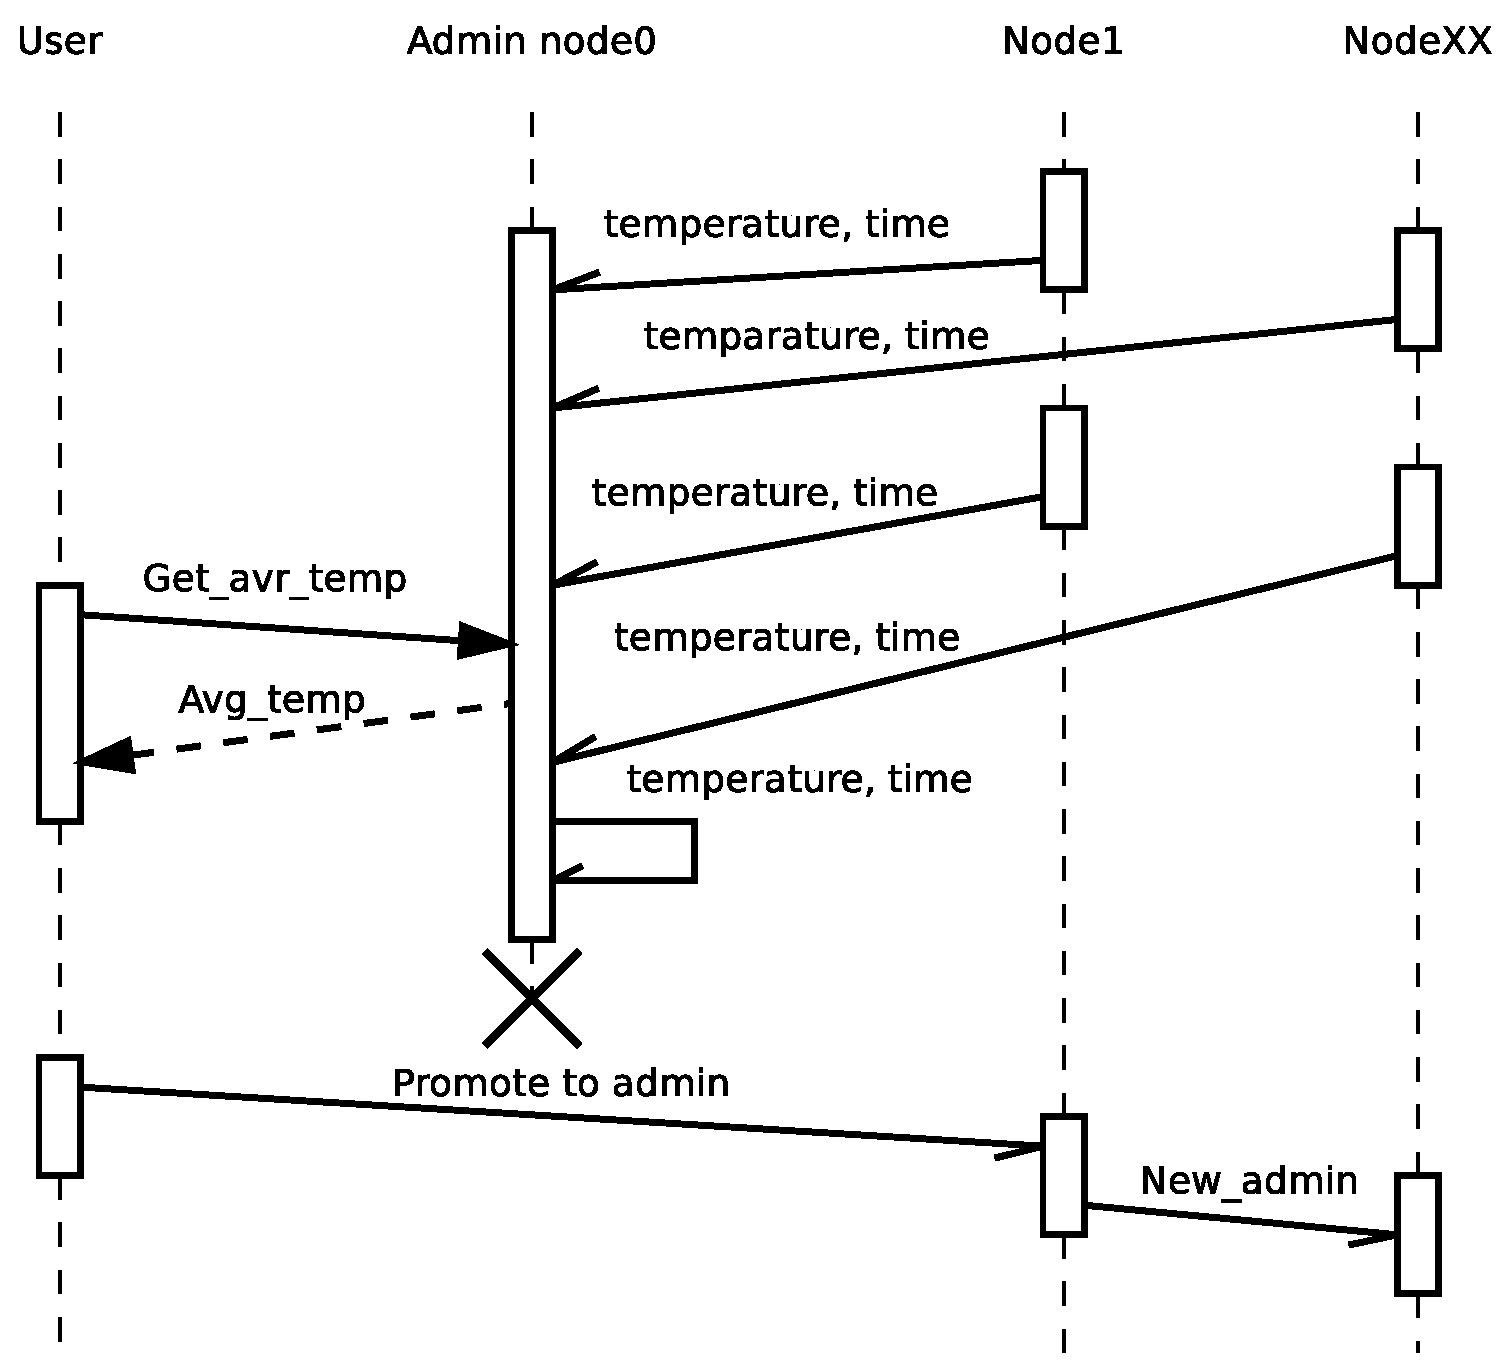
\includegraphics[scale=0.4]{eps/communications2}
\caption{The most prominent messages in the system}
\label{fig:overview}
\end{figure}
\subsection{Assumptions}
\label{subsec:assumptions}
The following assumptions are made about the context of the system:
\begin{itemize}
    \item All nodes are syncronized within a certain margin. This is done to be able to timestamp each temperature value and provide the user with an up to date picture of the temperature situation. 
    \item Reliable channels. Using the TCP protocol each data point is assumed delivered after it has been sent. % [Come up with a justification]
    \item Secure channels. No data is corrupted or generated by outsiders with malicious intend.
    \item Data integrity. The data received is assumed to be the data that is sent. No data is generated out of nowhere.
    \item IP addresses of all nodes are known to the user in before deployment of each node.
    \item Channels are asynchronous and message can take arbitrary time to arrive.
    %\item mode assumptions...?
\end{itemize}
